\chapter{NTT training details}
\label{app:a}

We present here further specifics about the choices made during pre-training and fine-tuning our NTT architecture. We also present the common hyper-parameters used for both. In the scope of our project, we do not perform a search to find the best performing hyper-parameters. Our objective is to explore what can be learnt, and not to achieve state-of-the-art results. The hyper-parameters for us are chosen based on Transformers trained in other domains, and with some tweaking, work reasonably well for our use case.

We implement our NTT in Python, using the PyTorch\cite{pytorch} and PyTorch Lightning\cite{pytorchlit} libraries. We implement our NTT in a Debian $10$ environment. For our training process, we use NVIDIA\textsuperscript{\textregistered} Titan Xp GPUs, with $12$ GB of GPU memory. For pre-training and fine-tuning on the full datasets, we use 2 GPUs with PyTorch's DataParallel implementation. For pre-processing our data, generating our input sliding window sequences and converting our data into training, validation and test batches, we use $4$ Intel\textsuperscript{\textregistered} $2.40$ GHz Dual Tetrakaideca-Core Xeon E5-2680 v4 CPUs and   between $60-80$ GB of RAM. 

\begin{table}[htbp]
\centering
\begin{tabular}{ l   c  }
\toprule
\emph{Hyper-parameter} & Value  \\
                                                       
\midrule
 Learning rate                                         &     $1\times10^{-4}$           \\
 Weight decay					  &       $1\times10^{-5}$          \\
 \# of attention heads 			  &          $8$      \\
 \# of Transformer layers			  &          $6$        \\
 Batch size 			  		&            $64$      \\
 Dropout prob.					&            $0.2$   \\
 Pkt. embedding dim.			&                   $120$     \\
    
\bottomrule

\end{tabular}
\caption{Hyper-parameters for NTT training}
\label{app:table1}
\end{table}

We refer to Table \ref{app:table1} to discuss our training hyper-parameters. The number of attention heads refers to the number of attention matrices used inside the Transformer encoder layers, which are processed in parallel. In our NTT architecture (Figure \ref{fig:ntt}), we have $691K$ trainable parameters from the embedding and aggregation layers, $3.3M$ trainable parameters from the Transformer encoder layers and $163K$ trainable parameters from linear layers in the decoder. We use $4$ linear layers in the decoder, with activation and layer-weight normalisation\cite{layernorm} between each linear layer.  We also use a layer-weight normalisation layer, as a pre-normalising layer, on the output of the embedding and aggregation. During training, we use a dropout probability\cite{dropout} of $0.2$ and a weight decay\cite{weightdecay} over the weights (not biases)\cite{goodfellowDeepLearning2016}, in order to prevent overfitting. We use a batch size of $64$, to reduce the noise during our training process.

We use the ADAM\cite{adam} optimiser with $\beta_1=0.9$, $\beta_2=0.98$ and $\epsilon=1\times10^{-9}$, for our training and the Huber loss\cite{huber} function for training loss (\ref{eq:huber}), as it is not super-sensitive to outliers but neither ignores their effects entirely. The loss function is computed on the residual \ie the difference between the observed  and predicted values, $y$ and $f(x)$ respectively.
\begin{equation}
L_\delta(y, f(x))=
    \begin{cases}
        \frac{1}{2}(y - f(x))^2 & \text{for } \lvert y - f(x) \rvert \leq \delta, \\
        \delta  \cdot (\lvert y - f(x) \rvert - \frac{1}{2}\delta) & \text{otherwise}
    \end{cases}
\label{eq:huber}
\end{equation}

We use a warm-up scheduler over our base learning rate (lr) of  $1\times10^{-4}$, as mentioned in the original Transformer paper\cite{vaswaniAttentionAllYou2017}. We present the governing equation for that as (\ref {eq:lr})

\begin{equation}
lr = d_{model}^{-0.5} \cdot \min{(step\_num^{-0.5}, warmup\_steps^{-0.5})}
\label{eq:lr}
\end{equation}

This corresponds to increasing the learning rate linearly for the first \emph{warmup\_steps} training steps, and decreasing it thereafter proportionally to the inverse square root of the step number. We used $warmup\_steps = 4000$ and our pre-training data has ${\sim}17K$ steps, and our $d_{model}$ is $120$.


\chapter{Learning with multiple decoders}
\label{app:b}

In Section \ref{ssec:impptt}, we evaluated the idea of masking different positions in the input sequence, in order to improve the pre-training phase of the NTT.  During this, we realised that with a variable masking approach, it is not always feasible to have a single set of linear layers to effectively act a combined MLP decoder, across all levels of aggregation. We present some further results on using different instances of identical MLP decoders, for different levels of aggregation, which are due to selecting the packet delays to be masked in different ways for pre-training. We summarise our findings in Table \ref{app:table2}.

\begin{table}[htbp]
\centering
\begin{tabular}{ l   c  }
\toprule
\emph{all values $\times10^{-3}$} & Pre-training \\
(Masking + MLP instance) & (Delay)  \\
                                                       
\midrule
\em{NTT: Chosen mask}                                              & 		 	 \\
\smallindent From encoded states + 1 MLP decoder                                         &      0.063         \\
\smallindent From encoded states + 3 MLP decoders                                         &     0.070          \\
\smallindent From aggregation levels + 1 MLP decoder  					&     1.31          \\
\smallindent  From aggregation levels + 3 MLP decoders  					&     0.087          \\
 
    
\bottomrule

\end{tabular}
\caption{MSE on delay prediction across NTT with multiple instances of linear MLP decoders}
\label{app:table2}
\end{table}

Based on our experiments, it is evident that we will need different instances of MLP decoders, when we mask across different levels of aggregation, with varying frequency of masking. In the case, where we choose from \emph{the encoded states}, we only choose the packets which are aggregated twice $1/48$ of the times, the packets which are aggregated once $15/48$ of the times, and hence we mainly choose the non-aggregated packets \ie $32/48$ of the times. In this scenario, it doesn't hurt the performance even if we use a single set of linear layers to extract the learnt behaviour across levels of aggregation, as most of the times, the non-aggregated packets are chosen. In this case, using a single MLP decoder vs using $3$ MLP decoders for learning has very similar performance.

When we choose from \emph{aggregation levels}, the situation is very different as every type of aggregation is chosen $1/3$ of the times. Effectively this results in the fact, that we mask $1/2$ of the packet delays, which are aggregated twice, $1/3$ of the times. In this scenario, a single MLP decoder cannot effectively learn across levels of aggregation, all of which are chosen frequently and in this case, using multiple MLP decoders, helps the learning process. A-priori, we do not know what kind of architecture works best for this, and thus we start with the simplest model, where we use three identical sets of linear layers, to match the independent levels of aggregation.

Based on the fact that different aggregation schemes may be used in future version of the NTT, different numbers of MLP decoders will be needed. One can certainly be sure that, with increasing complexity and aggregation, more complexity will also be required in the decoder architecture, to learn newer kinds of information.

\chapter{Delay distributions on the multi-path topology}
\label{app:c}

We present further insights in this section, about the individual delay distributions seen on each end-to-end path (from sending sources to each individual receiver) as shown in Figure \ref{fig:topo_ft_big}. A-priori, we should not assume that increasing complexity in traffic flows on the network, changes the traffic distributions on each individual path. Our NTT learns dynamics only on a single path during pre-training. We hypothesise that this can generalize to topologies with different paths and different dynamics with fine-tuning. For this we should try to check for the case, when these delay dynamics on different paths (affected by queueing delay and link delay) are different.

\begin{figure*}[!h]
  \begin{center}
    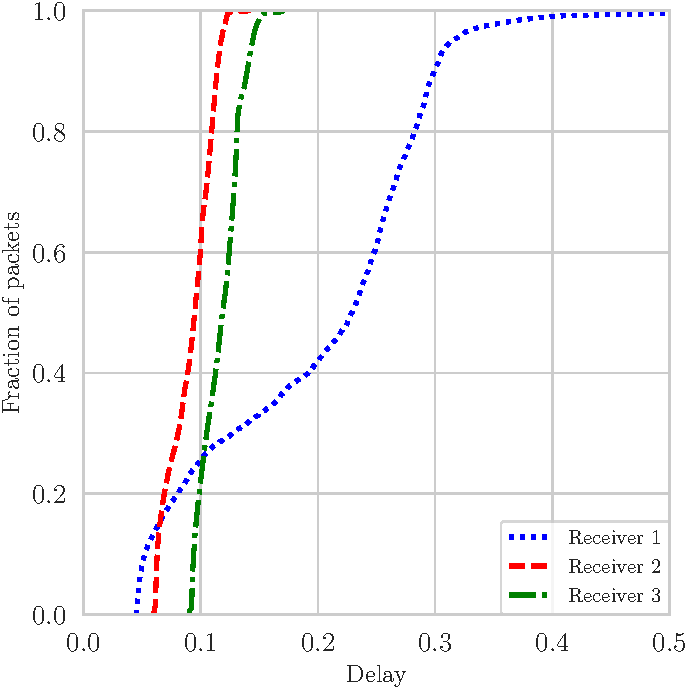
\includegraphics[scale=0.8]{figures/delay_Receivers.pdf}
    \caption{Comparing delay CDFs across multiple paths}
    \label{fig:multipatht}
  \end{center}
\end{figure*}

We can see in Figure \ref{fig:multipatht} that the network dynamics change considerably, as we increase the paths in the network, as we compare the CDFs of the packet delays at all receivers. We observe that the dynamics change a lot from the path to Receiver 1 to the path to Receiver 2, but in our setup, not so much in the paths to Receiver 2 and Receiver 3. IWe can clearly see from the experimental results in the Section \ref{ssec:comptop}, that the pre-trained NTT generalizes to newer topologies with varying dynamics across different paths. However, for testing the NTT in a more robust manner, it is evident that we need to fine-tune on multiple topologies, with different path dynamics in order to check the true extent of generalization. For the purpose of this thesis, such evaluation is not in the current scope and we leave that to future experiments.

\chapter{Declaration of Originality}
\label{app:d}

Placeholder for signed Declaration of Originality.

